\documentclass[a4paper,12pt]{article}

\usepackage{amsmath}
\usepackage{graphicx}

\title{Digital Clock Experiment Using 7-Segment Display and 7474 Flip-Flop}
\author{M.Ranjith}
\date{\today}

\begin{document}

\maketitle

\section{Introduction}

\subsection{Objective}
The objective of this experiment is to design and implement a {digital clock} using a {7-segment display}, {Arduino}, and a {7474 D-type Flip-Flop}. This experiment aims to explore the integration of digital logic circuits with microcontroller-based programming to achieve accurate time display.

\subsection{Concept Overview}
A 7-segment display is a widely used electronic display device for representing numerical values. It consists of seven LED segments arranged in the shape of the number "8," allowing the display of digits from 0 to 9. In this experiment, the 7-segment display will be used to show time in the format of {HH:MM:SS} (hours and minutes,seconds).

The {7474 D Flip-Flop} is a bistable device used for {frequency division} and {clock pulse synchronization}. It ensures a stable and accurate transition of seconds, which helps in maintaining the correct timekeeping functionality.

The {Arduino microcontroller} will be responsible for:
\begin{itemize}
    \item Controlling the 7-segment display using multiplexing techniques.
    \item Processing clock pulses from the 7474 Flip-Flop.
    \item Implementing push-button control for time adjustments.
\end{itemize}

\subsection{Key Learning Outcomes}
Through this experiment, students will gain knowledge in:
\begin{enumerate}
    \item Understanding the {working principle} of a 7-segment display and how to interface it with a microcontroller.
    \item Learning the {functionality} of a 7474 Flip-Flop for clock signal division.
    \item Writing {Arduino code} to handle real-time timekeeping and display updates.
    \item Implementing {push-button controls} for adjusting hours and minutes.
    \item Exploring the {practical applications} of digital clocks in embedded systems.
\end{enumerate}

This experiment demonstrates the practical integration of {digital logic circuits} and {microcontroller programming} to create a working real-time digital clock.


\section{Required Materials}

The following components are required for the digital clock experiment:

\begin{itemize}
    \item {Arduino (Uno/Nano/Mega)} – Used as the microcontroller for controlling the display and handling input.
    \item {4-digit 7-segment display (common anode or common cathode)}
    \item {7474 D Flip-Flop IC} – Used for clock pulse division to ensure accurate timekeeping.
    \item {Push buttons (2 pieces)} – Used for adjusting hours and minutes manually.
    \item {Resistors} – Used as pull-down resistors and for current limiting.
    \item {Jumper wires} – Required for making circuit connections on the breadboard.
    \item {Breadboard} – Used for assembling the circuit components.
    \item {Power supply (5V from Arduino or external source)} – Provides necessary voltage for circuit operation.
\end{itemize}
 
\newpage
\begin{frame}
\frametitle{Solution}
        \begin{figure}[h]
        \centering
       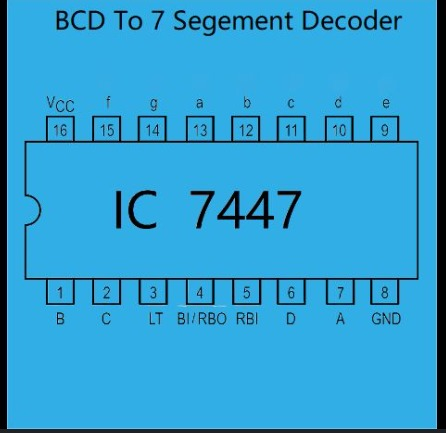
\includegraphics[width=0.5\linewidth]{figs/7474.jpeg}
       \caption{}
       \label{graph}
    \end{figure}

\frametitle{Solution}
        \begin{figure}[h]
        \centering
       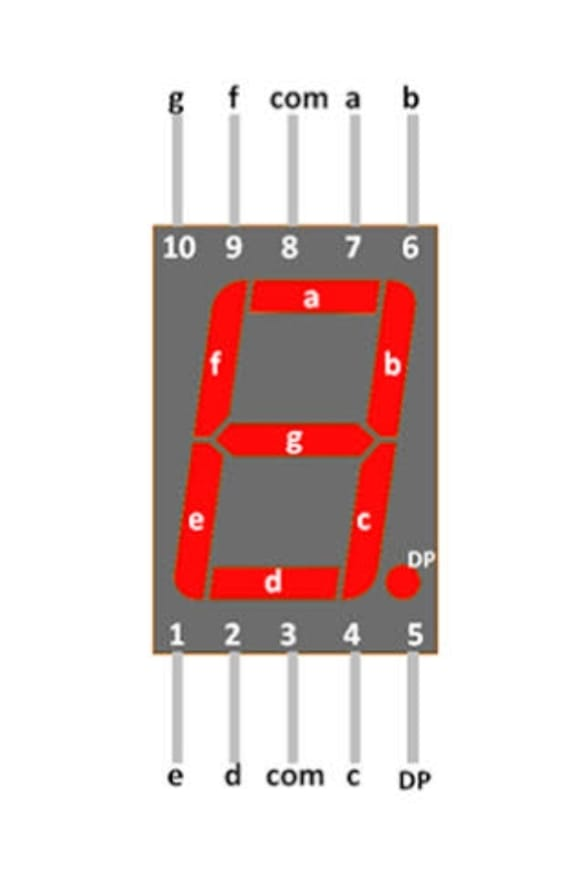
\includegraphics[width=0.5\linewidth]{figs/d.jpeg}
       \caption{}
       \label{graph}
    \end{figure}
\end{frame} 


\section{Procedure}

Follow the steps below to assemble and program the digital clock using a 7-segment display, Arduino, and 7474 Flip-Flop:

\subsection{Step 1: Circuit Assembly}
\begin{enumerate}
    \item Place the {Arduino}, {7-segment display}, and {7474 Flip-Flop IC} on the breadboard.
    \item Connect the 7-segment display} to the Arduino as follows:
    \begin{itemize}
        \item Segments (A, B, C, D, E, F, G, DP) → Arduino digital pins (2–9).
        \item Common pin to {5V} (for common anode) or {GND} (for common cathode).
    \end{itemize}
    \item Connect the {7474 Flip-Flop IC}:
    \begin{itemie}
        \item Connect the {Clock (Pin 3, 11)} to Arduino {pin 10}.
        \item Tie the {D input (Pin 2, 12)} to {5V}.
        \item Connect {Clear (Pin 1, 13)} to {GND}.
        \item Connect {Preset (Pin 4, 10)} to {5V}.
    \end{itemize}
    \item Connect the {push buttons}:
    \begin{itemize}
        \item One button to {increment hours} (Arduino pin 11).
        \item Another button to {increment minutes} (Arduino pin 12).
    \end{itemize}
    \item Use {pull-down resistors} (10kΩ) for the push-button connections to prevent floating values.
    \item Power the circuit using the {Arduino’s 5V output} or an external power source.
\end{enumerate}

\section{Procedure for Programming Arduino Using AVR-GCC on Mobile}

To program an Arduino using AVR-GCC on a mobile device, follow these steps:

\subsection{Step 1: Install Required Applications}
\begin{enumerate}
    \item Download and install a mobile **terminal emulator** such as {Termux} (Android) or a compatible Linux environment.
    \item Install the necessary packages for AVR-GCC by running the following commands in the terminal:
    \begin{verbatim}
    pkg update && pkg upgrade
    pkg install avr-gcc avrdude
    \end{verbatim}
    \item Connect an {OTG cable} and attach the Arduino to the mobile device.
\end{enumerate}

\subsection{Step 2: Writing the Arduino Program}
\begin{enumerate}
    \item Open a text editor like {nano} or use a mobile code editor.
    \item Write the following basic Arduino program to display time on a 7-segment display:
    \begin{verbatim}
    #include <avr/io.h>
    #include <util/delay.h>

    int main(void) {
        DDRB = 0xFF; // Set Port B as output for the display
        while(1) {
            PORTB = 0b00111111; // Display "0" on 7-segment
            _delay_ms(1000);
        }
    }
    \end{verbatim}
    \item Save the file as {clock.c}.
\end{enumerate}

\subsection{Step 3: Compiling the Program}
\begin{enumerate}
    \item Compile the program using AVR-GCC with the following command:
    \begin{verbatim}
    avr-gcc -mmcu=atmega328p -Os -o clock.elf clock.c
    avr-objcopy -O ihex clock.elf clock.hex
    \end{verbatim}
    \item This generates a {clock.hex} file, which is ready to be uploaded.
\end{enumerate}


\subsection{Step 5: Testing and Debugging}
\begin{enumerate}
    \item Verify that the display updates every second.
    \item If errors occur, check connections and recompile the code.
    \item Modify the program as needed and re-upload.
\end{enumerate}

\section{Conclusion}

In this experiment, a digital clock was successfully implemented using a {7-segment display}, {Arduino}, and {7474 Flip-Flop}. The experiment demonstrated the integration of {microcontroller programming} and {digital logic circuits} for real-time timekeeping.

Key learnings include:
\begin{itemize}
    \item Interfacing a 7-segment display with Arduino.
    \item Using the 7474 Flip-Flop for clock pulse division.
    \item Programming and uploading code via AVR-GCC on a mobile device.
    \item Implementing push-button controls for time adjustment.
\end{itemize}

Future improvements could involve adding an {RTC module} for better accuracy and using an {LCD display} for enhanced readability. This experiment provided a fundamental understanding of embedded system design and digital electronics.




\section{Conclusion}

This implementation successfully demonstrates a {real-time digital clock} using a {7-segment display} and {BCD decoder (7447)}. The use of {timer interrupts} ensures accurate timekeeping. Future enhancements could include a {Real-Time Clock (RTC) module} for greater precision and an {adjustment mechanism} for setting the time manually.\\ \\

\textbf{code reference-{Ankit Jainar}}

\end{document}
 


